% --- ETUDE DE CAS ---
\newpage
\section*{Étude de cas~: Architecture Big Data}
\phantomsection
\addcontentsline{toc}{section}{Étude de cas~: Architecture Big Data}

\subsection*{AAV}
\phantomsection
\addcontentsline{toc}{subsection}{AAV}
\begin{itemize}
	\item [1] Identifier les contraintes sur les données liées au RGPD
	\item [2] Interpréter les 5V du Big Data
	\item [2] Décrire une architecture Big Data
	\item [2] Décrire une infrastructure de stockage distribuée (cluster de serveurs, virtualisation, NAS vs SAN, \dots)
	\item [2] Décrire l'utilisation du cloud dans le cadre du stockage de données
	\item [3] Présenter le traitement de données de manière distribuée (exemple~: MapReduce)
	\item [2] Décrire le fonctionnement des systèmes de fichiers distribués
	\item [2] Décrire le fonctionnement d'une application d'entreposage de données
	\item [3] Concevoir un modèle dimensionnel (Data Mart)
	\item [1] Identifier les difficultés associées aux traitements distribués
\end{itemize}

\subsection*{Rôles}
\phantomsection
\addcontentsline{toc}{subsection}{Rôles}
\begin{itemize}
	\item Animateur~: Stéphane
	\item Secrétaire / Scribe~: Marine
	\item Gestionnaire~: Victor
\end{itemize}

\subsection*{Mots clés}
\phantomsection
\addcontentsline{toc}{subsection}{Mots clés}
\begin{itemize}
	\item Big Data
	\item CHU
	\item Entrepôt de données
	\item Data Lake
	\item Cloudera
	\item Power BI
	\item RGPD
	\item Données multidimensionnelles
	\item Environnement virtualisé
	\item Modélisation des données
	\item Outil de planification
\end{itemize}

\subsection*{Contexte}
\phantomsection
\addcontentsline{toc}{subsection}{Contexte}
\noindent Votre équipe reprend le projet du groupe CHU (\textit{Cloud Healthcare Unit}). Vous disposez de 3 semaines pour livrer une maquette complète d'entrepôt de données décisionnel pour le secteur hospitalier en repartant du schéma d'architecture Big Data et du modèle logique.

\subsection*{Problématique}
\phantomsection
\addcontentsline{toc}{subsection}{Problématique}
\noindent Comment valider une architecture Big Data performante et concevoir le modèle logique d'un entrepôt de données décisionnel adapté aux données personnelles du projet CHU~?

\subsection*{Contraintes}
\phantomsection
\addcontentsline{toc}{subsection}{Contraintes}
\begin{itemize}
	\item Temps (2 jours)
	\item Budget
	\item L'existant (schéma d'architecture~; les données)
	\item Performances / Volumétrie
	\item Conformité / Légalité
\end{itemize}

\subsection*{Généralisation}
\phantomsection
\addcontentsline{toc}{subsection}{Généralisation}
\begin{itemize}
	\item Big Data
	\item Architecture
	\item Datawarehouse
	\item Data Lake
	\item Virtualisation
	\item Cloud
	\item Cloudera
	\item Power BI
	\item Stockage
	\item Modélisation
	\item RGPD
\end{itemize}

\subsection*{Livrables}
\phantomsection
\addcontentsline{toc}{subsection}{Livrables}
\begin{itemize}
	\item Une maquette d'architecture répondant aux besoins du projet
	\item Modèle logique / conceptuel de données
\end{itemize}

\subsection*{Pistes de solutions}
\phantomsection
\addcontentsline{toc}{subsection}{Pistes de solutions}
\begin{itemize}
	\item Se renseigner sur les styles d'architecture Big Data, le stockage distribué, les systèmes de fichiers distribués, les Data Lakes et l'évolution des architectures décisionnelles.
	\item Étudier le schéma de l'architecture produit par Archie et faire le lien avec les outils présents dans l'environnement virtualisé (comme Cloudera et Power BI).
	\item Explorer les fichiers de données situés dans le dossier «~Mes documents~» afin d'identifier les informations répondant aux analyses du cahier des charges.
	\item Appliquer les principes des bases de données multidimensionnelles et de l'entre\-po\-sage de données (Datawarehouse) pour démarrer la modélisation logique en parallèle.
	\item Se renseigner sur la protection des données à caractère personnel via la ressource «~Data et RGPD~» ainsi que sur les métiers de la data science.
\end{itemize}

\subsection*{Plan d'actions}
\phantomsection
\addcontentsline{toc}{subsection}{Plan d'actions}
\begin{itemize}
	\item Définir les mots clés liés au Big Data, à l'entreposage de données décisionnel et au RGPD.
	\item Étudier les ressources fournies sur l'architecture Big Data, le Datawarehouse, le Data Lake, la virtualisation, le stockage distribué et le RGPD.
	\item Analyser le schéma de l'architecture d'Archie et inspecter l'environnement virtualisé mis en place.
	\item Parcourir les données du dossier «~Mes documents~» en identifiant les données personnelles et les besoins d'analyse décrits dans le cahier des charges.
	\item Concevoir en parallèle la modélisation des données (modèle logique multidimensionnel) pour répondre aux exigences de performance.
	\item Valider le choix de l'architecture et le modèle logique dans le délai de 2 jours afin de préparer les phases suivantes (intégration, implémentation physique, exploitation et visualisation).
\end{itemize}

\newpage
% --- DEFINITIONS ---
\newpage
\section{Définitions des mots clés}

\needspace{8\baselineskip}
\noindent \textbf{Big Data}:
\noindent Le Big Data désigne des ensembles de données si volumineux, rapides ou variés qu'ils dépassent les capacités des outils de stockage et de traitement traditionnels (SGBD relationnel sur un seul serveur). On le caractérise classiquement par les \textbf{5 V}~:
\begin{itemize}
	\item \textbf{Volume}~: des quantités de données massives (téraoctets, pétaoctets) ;
	\item \textbf{Vélocité}~: des données produites et à traiter rapidement, parfois en temps réel ;
	\item \textbf{Variété}~: des données structurées (tables), semi-structurées (JSON, XML, CSV) et non structurées (textes, images médicales) ;
	\item \textbf{Véracité}~: la fiabilité et la qualité des données, à vérifier avant exploitation ;
	\item \textbf{Valeur}~: l'intérêt métier que l'on peut tirer de l'analyse des données.
\end{itemize}
Pour y répondre, on distribue le stockage et les calculs sur un ensemble de machines (cluster) plutôt que d'augmenter la puissance d'un seul serveur.

\begin{center}
\begin{tikzpicture}[
  v/.style={circle,draw=title1,fill=title2!15,thick,minimum size=2.2cm,align=center,font=\small\bfseries}]
  \node[circle,fill=title1,text=white,minimum size=2.4cm,font=\bfseries] (c) {Big Data};
  \foreach \n/\a [count=\i] in {Volume/90,Vélocité/18,Variété/-54,Véracité/-126,Valeur/162} {
    \node[v] (v\i) at (\a:3.3cm) {\n};
    \draw[thick,title1] (c) -- (v\i);
  }
\end{tikzpicture}
\end{center}

\separateur

\needspace{8\baselineskip}
\noindent \textbf{CHU}:
\noindent Dans le sujet, CHU désigne le groupe \textit{Cloud Healthcare Unit}, client du projet, qui souhaite disposer d'un entrepôt de données décisionnel pour le secteur hospitalier. Le terme renvoie aussi aux Centres Hospitaliers Universitaires, établissements qui produisent un grand volume de données de santé (patients, consultations, hospitalisations, actes, prescriptions). Ces données sont sensibles et soumises à une réglementation stricte.

\separateur

\needspace{8\baselineskip}
\noindent \textbf{Entrepôt de données (Data Warehouse)}:
\noindent Un entrepôt de données est une base de données dédiée à l'analyse et à la prise de décision. Selon la définition de Bill Inmon, ses données sont~:
\begin{itemize}
	\item \textbf{orientées sujet}~: organisées autour des thèmes métier (patients, séjours, actes) ;
	\item \textbf{intégrées}~: issues de sources multiples puis harmonisées ;
	\item \textbf{non volatiles}~: les données chargées ne sont ni modifiées ni supprimées ;
	\item \textbf{historisées}~: conservées dans le temps pour suivre les évolutions.
\end{itemize}
Il est alimenté par un processus ETL (\textit{Extract, Transform, Load}) et peut être découpé en \textbf{Data Marts}, des sous-ensembles dédiés à un service ou à un besoin d'analyse précis.

\separateur

\needspace{8\baselineskip}
\noindent \textbf{Data Lake}:
\noindent Un Data Lake (lac de données) est un espace de stockage qui conserve de grandes quantités de données \textbf{brutes}, dans leur format d'origine, qu'elles soient structurées ou non. Contrairement à l'entrepôt, le schéma n'est appliqué qu'au moment de la lecture (\textit{schema-on-read}). Il repose généralement sur un système de fichiers distribué (HDFS) ou un stockage objet dans le cloud.

\begin{center}
\begin{tabularx}{\textwidth}{>{\bfseries}l X X}
\toprule
 & Data Warehouse & Data Lake \\
\midrule
Données & Structurées, nettoyées & Brutes, tous formats \\
Schéma & À l'écriture (\textit{schema-on-write}) & À la lecture (\textit{schema-on-read}) \\
Usage & Reporting, tableaux de bord, OLAP & Exploration, data science, archivage \\
Utilisateurs & Décideurs, analystes métier & Data scientists, data engineers \\
\bottomrule
\end{tabularx}
\end{center}

Les deux sont complémentaires~: le Data Lake sert souvent de zone d'atterrissage avant l'alimentation de l'entrepôt.

\separateur

\needspace{8\baselineskip}
\noindent \textbf{Cloudera}:
\noindent Cloudera est un éditeur qui fournit une distribution de l'écosystème \textbf{Apache Hadoop} (CDH, puis Cloudera Data Platform). Elle regroupe et administre les principaux outils Big Data~:
\begin{itemize}
	\item \textbf{HDFS}~: système de fichiers distribué qui découpe et réplique les fichiers sur les nœuds du cluster ;
	\item \textbf{YARN} et \textbf{MapReduce}~: gestion des ressources et traitement distribué ;
	\item \textbf{Hive} et \textbf{Impala}~: interrogation des données en SQL ;
	\item \textbf{HBase}~: base NoSQL orientée colonnes ;
	\item \textbf{Sqoop}~: import/export entre bases relationnelles et Hadoop ;
	\item \textbf{Hue}~: interface web pour manipuler ces outils.
\end{itemize}

Dans le projet, Cloudera constitue la couche de stockage et de traitement de l'archi\-tec\-ture.

\separateur

\begin{wrapfigure}{r}{0.18\textwidth}
    \vspace{-20pt}
    \begin{center}
        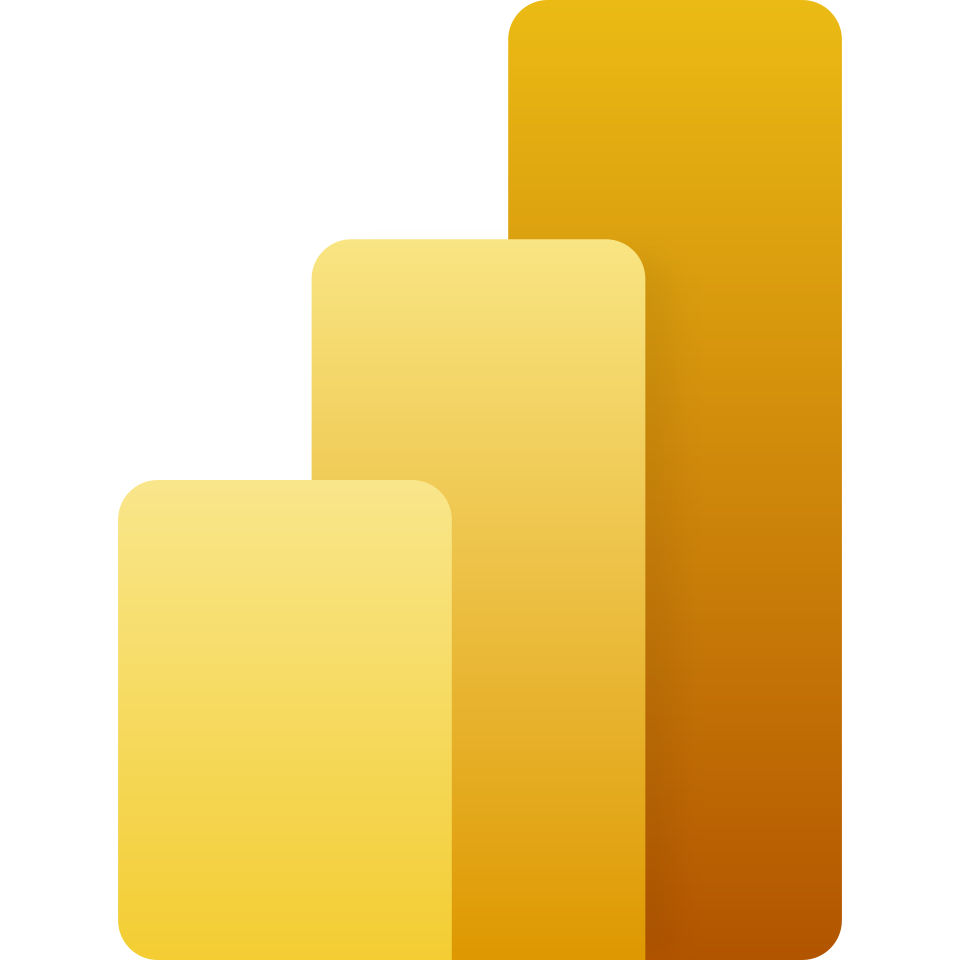
\includegraphics[width=0.13\textwidth]{contents/img/logo_powerbi.png}
    \end{center}
    \vspace{-15pt}
\end{wrapfigure}

\needspace{8\baselineskip}
\noindent \textbf{Power BI}:
\noindent Power BI est l'outil de \textit{Business Intelligence} de Microsoft. Il se connecte à de nombreuses sources (dont Hive et Impala), permet de modéliser les données et de construire des tableaux de bord interactifs. Dans l'architecture, il forme la couche de restitution~: il présente aux décideurs du CHU les indicateurs (KPI) calculés à partir de l'entrepôt.

\separateur

\needspace{8\baselineskip}
\noindent \textbf{RGPD}:
\noindent Le Règlement Général sur la Protection des Données (UE 2016/679), applicable depuis le 25 mai 2018, encadre le traitement des données à caractère personnel. Les données de santé y sont classées comme \textbf{données sensibles}~: leur traitement est interdit sauf exceptions encadrées. Principes à respecter dans le projet~:
\begin{itemize}
	\item \textbf{licéité et finalité}~: traiter les données pour un objectif défini et légitime ;
	\item \textbf{minimisation}~: ne conserver que les données nécessaires aux analyses ;
	\item \textbf{limitation de la conservation}~: définir une durée de conservation ;
	\item \textbf{sécurité}~: contrôle des accès, chiffrement, traçabilité ;
	\item \textbf{pseudonymisation / anonymisation}~: retirer ou remplacer les identifiants directs (nom, numéro de sécurité sociale).
\end{itemize}
En France, l'hébergement de données de santé doit en plus être confié à un hébergeur certifié HDS, et la CNIL contrôle le respect du règlement.

\separateur

\needspace{8\baselineskip}
\noindent \textbf{Données multidimensionnelles}:
\noindent Les données multidimensionnelles sont organisées pour l'analyse selon plusieurs axes. Elles reposent sur deux notions~:
\begin{itemize}
	\item \textbf{les faits}~: les mesures à analyser, souvent numériques (nombre de consultations, durée de séjour, coût) ;
	\item \textbf{les dimensions}~: les axes d'analyse (temps, patient, établissement, diagnostic, professionnel de santé).
\end{itemize}
Cette organisation forme un \textbf{cube OLAP} que l'on peut explorer par agrégation (\textit{roll-up}), détail (\textit{drill-down}), découpage (\textit{slice}, \textit{dice}) ou pivot.

\begin{center}
  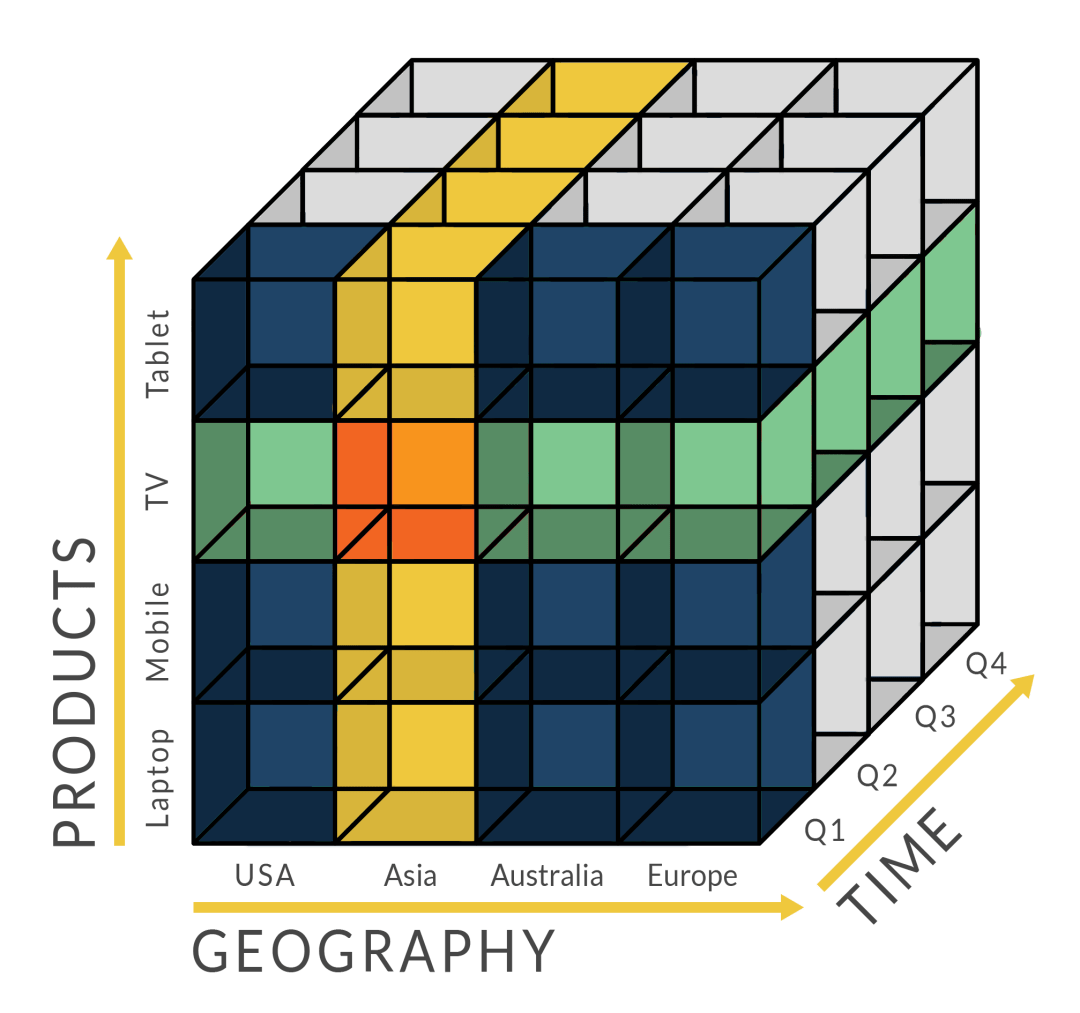
\includegraphics[width=0.33\textwidth]{contents/img/cube_olap.png}
\source{Wikimedia Commons, \textit{Olap-3d-cube.png} (CC BY-SA 4.0)}
\end{center}

\separateur

\needspace{8\baselineskip}
\noindent \textbf{Environnement virtualisé}:
\noindent Un environnement virtualisé est un ensemble de machines virtuelles exécutées sur une même machine physique grâce à un hyperviseur (VMware, VirtualBox, Hyper-V). Dans le projet, il héberge les outils de la maquette (Cloudera, Power BI) et les fichiers de données. Il permet de reproduire l'architecture cible à moindre coût, de l'isoler et de la remettre en état facilement (instantanés).

\separateur

\needspace{8\baselineskip}
\noindent \textbf{Modélisation des données}:
\noindent La modélisation consiste à décrire la structure des données avant de les implémenter, à plusieurs niveaux (conceptuel, logique, physique). Pour un entrepôt, on utilise une modélisation dimensionnelle, qui organise les données en faits et en dimensions. Les différents modèles sont étudiés dans la partie~\ref{sec:modelisation}.

\separateur

\needspace{8\baselineskip}
\noindent \textbf{Outil de planification}:
\noindent Un outil de planification sert à organiser le projet dans le temps~: découper le travail en tâches, estimer leur durée, identifier les dépendances et répartir les responsabilités. Exemples~: diagramme de Gantt (MS Project, GanttProject), tableau Kanban (Trello, Jira). Avec trois semaines pour livrer la maquette, il permet de suivre l'avancement de chaque phase (architecture, intégration, implémentation, visualisation).

% --- INFRASTRUCTURE ---
\newpage
\section{Infrastructure et traitement distribués}

\subsection{Cluster de serveurs et virtualisation}

\needspace{8\baselineskip}
\noindent \textbf{Cluster de serveurs}:
\noindent Un cluster est un ensemble de serveurs (\textbf{nœuds}) reliés en réseau qui travaillent comme un seul système. Face à l'augmentation des données, deux stratégies existent~:
\begin{itemize}
	\item \textbf{scalabilité verticale} (\textit{scale up})~: ajouter de la puissance (CPU, RAM, disques) à un seul serveur. Simple, mais limité et coûteux ;
	\item \textbf{scalabilité horizontale} (\textit{scale out})~: ajouter des serveurs standards au cluster. C'est le principe du Big Data~: la capacité augmente de façon quasi linéaire avec le nombre de nœuds.
\end{itemize}
Le cluster apporte aussi la \textbf{tolérance aux pannes}~: les données étant répliquées, la perte d'un nœud n'interrompt pas le service.

\vspace{0.5cm}

\needspace{8\baselineskip}
\noindent \textbf{Virtualisation}:
\noindent La virtualisation permet de faire tourner plusieurs serveurs virtuels sur une même machine physique. Elle facilite le déploiement et la mutualisation des ressources (maquettes, environnements de test). Pour un cluster Big Data en production, on préfère souvent des machines physiques ou des conteneurs, car Hadoop repose sur la \textbf{localité des données}~: le calcul est envoyé sur le nœud qui stocke la donnée, ce qu'une couche de stockage virtualisée partagée peut fausser.

\subsection{Stockage~: DAS, NAS et SAN}

\begin{center}
  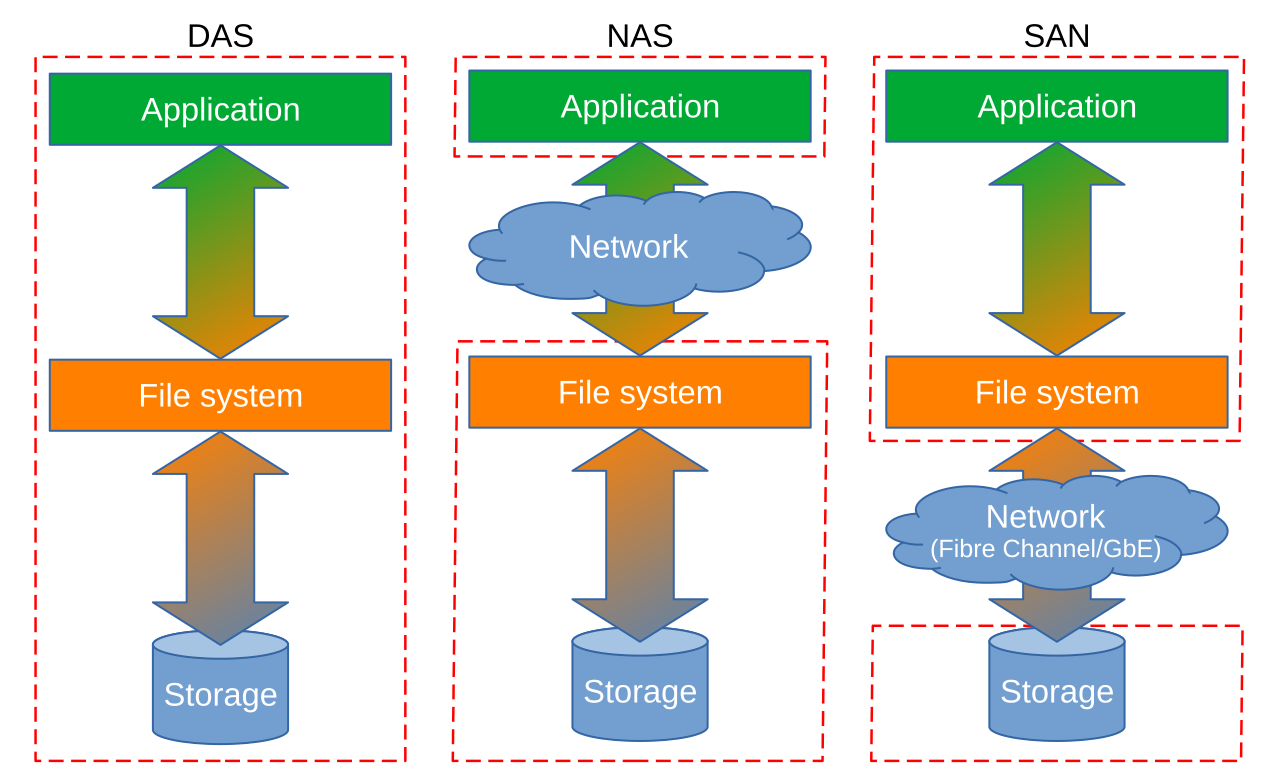
\includegraphics[width=0.75\textwidth]{contents/img/das_nas_san.png}
\source{Wikimedia Commons, Mattias Campe, \textit{DASvsNASvsSAN.svg} (CC BY-SA 4.0)}
\end{center}

\begin{center}
\begin{tabularx}{\textwidth}{>{\bfseries}l X X X}
\toprule
 & DAS & NAS & SAN \\
\midrule
Principe & Disques attachés directement au serveur & Serveur de fichiers partagé sur le réseau & Réseau dédié au stockage, vu comme des disques locaux \\
Accès & Bloc, local & Fichier (NFS, SMB/CIFS) & Bloc (Fibre Channel, iSCSI) \\
Réseau & Aucun & Réseau local (Ethernet) & Réseau dédié haut débit \\
Avantages & Simple, rapide, peu coûteux & Facile à partager, peu coûteux & Très performant, haute disponibilité \\
Inconvénients & Non partagé & Performances limitées par le réseau & Coûteux, complexe à administrer \\
Usage & Nœuds Hadoop (HDFS) & Partage de documents, sauvegardes & Bases de données critiques, virtualisation \\
\bottomrule
\end{tabularx}
\end{center}

\noindent Hadoop privilégie le DAS~: chaque nœud stocke ses propres blocs et HDFS assure lui-même le partage et la réplication, sans matériel de stockage coûteux.

\subsection{Le cloud pour le stockage de données}

\noindent Le cloud fournit des ressources informatiques à la demande, accessibles par le réseau et facturées à l'usage. On distingue trois modèles de service~:
\begin{itemize}
	\item \textbf{IaaS}~: le fournisseur met à disposition l'infrastructure (machines virtuelles, stockage, réseau) ;
	\item \textbf{PaaS}~: il fournit en plus une plateforme gérée (par exemple un cluster Hadoop ou un entrepôt managé) ;
	\item \textbf{SaaS}~: il fournit une application prête à l'emploi (Power BI Service).
\end{itemize}
Et trois modèles de déploiement~: \textbf{public} (ressources mutualisées chez un fournisseur), \textbf{privé} (dédié à une organisation) et \textbf{hybride} (combinaison des deux).

\begin{center}
  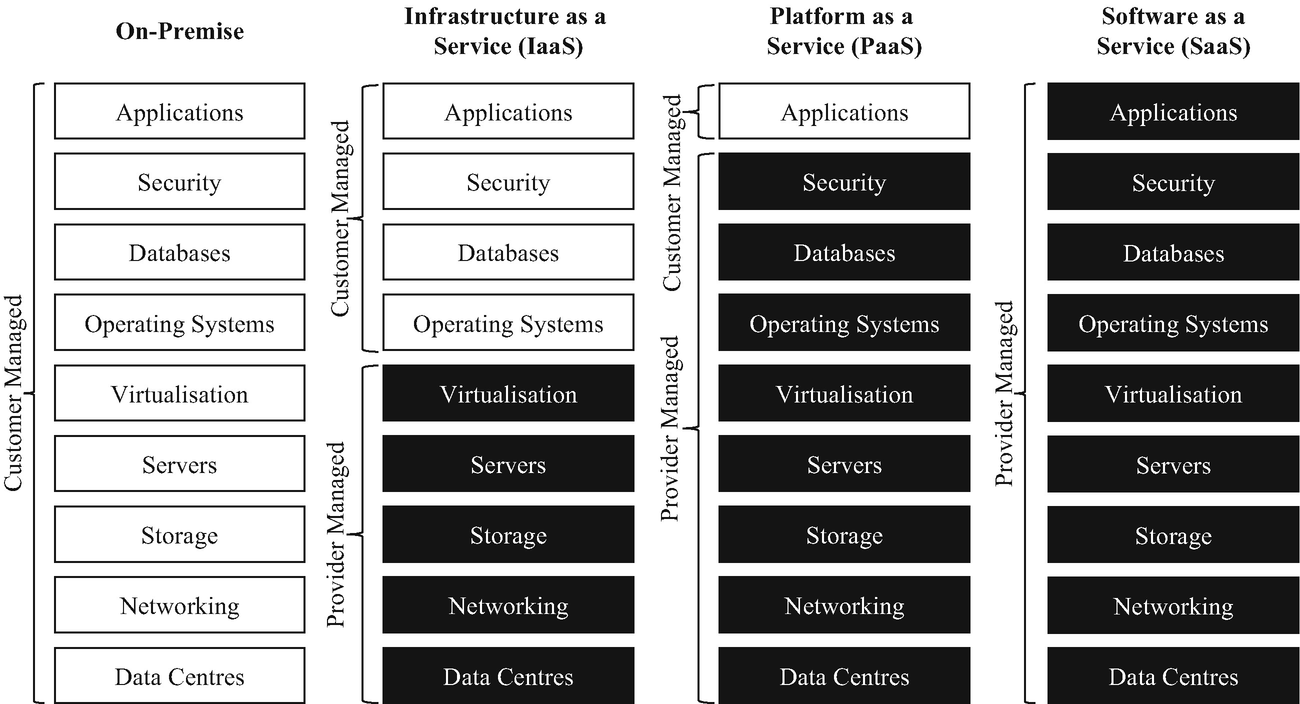
\includegraphics[width=0.72\textwidth]{contents/img/cloud_iaas_paas_saas.png}
\source{Wikimedia Commons, P. Rosati \& T. Lynn (domaine public). En noir~: ce que gère le fournisseur.}
\end{center}

\noindent Pour le stockage, le cloud propose notamment le \textbf{stockage objet} (Amazon S3, Azure Blob Storage, Google Cloud Storage), souvent utilisé comme Data Lake.

\begin{center}
\begin{tabularx}{\textwidth}{>{\raggedright\arraybackslash}X >{\raggedright\arraybackslash}X}
\toprule
\textbf{Avantages} & \textbf{Inconvénients} \\
\midrule
Élasticité~: capacité ajustée au besoin & Dépendance au fournisseur et au réseau \\
Pas d'investissement matériel initial & Coûts difficiles à prévoir sur de gros volumes \\
Haute disponibilité et réplication géographique & Localisation et confidentialité des données \\
Services managés (moins d'administration) & Conformité réglementaire à vérifier \\
\bottomrule
\end{tabularx}
\end{center}

\noindent Pour le CHU, les données de santé imposent un fournisseur certifié \textbf{HDS} et un hébergement compatible avec le RGPD (données dans l'Union européenne).

\subsection{Système de fichiers distribué~: HDFS}

\noindent Un système de fichiers distribué stocke les fichiers sur plusieurs machines tout en les présentant à l'utilisateur comme un système de fichiers unique. HDFS (\textit{Hadoop Distributed File System}) en est l'exemple de référence. Il repose sur une architecture maître/esclaves~:
\begin{itemize}
	\item \textbf{NameNode} (maître)~: gère l'arborescence et les métadonnées, c'est-à-dire la liste des blocs de chaque fichier et leur emplacement. Il ne stocke pas les données ;
	\item \textbf{DataNodes} (esclaves)~: stockent les blocs de données et envoient régulièrement un signal de vie (\textit{heartbeat}) au NameNode ;
	\item \textbf{Secondary / Standby NameNode}~: sauvegarde les métadonnées ou prend le relais en cas de panne du NameNode.
\end{itemize}

\noindent Fonctionnement~:
\begin{itemize}
	\item chaque fichier est découpé en \textbf{blocs} de grande taille (128~Mo par défaut) ;
	\item chaque bloc est \textbf{répliqué} (3 copies par défaut) sur des nœuds différents, en tenant compte des racks (\textit{rack awareness}) ;
	\item si un DataNode ne répond plus, le NameNode recrée les copies manquantes à partir des autres répliques ;
	\item le modèle est \textbf{\textit{write once, read many}}~: un fichier écrit n'est pas modifié, on y ajoute ou on le réécrit. Ce modèle est adapté aux lectures séquentielles de gros volumes.
\end{itemize}

\begin{center}
\begin{tikzpicture}[font=\small,
  box/.style={draw=title1,thick,rounded corners,align=center},
  blk/.style={draw,fill=#1,minimum width=0.7cm,minimum height=0.5cm,font=\scriptsize\bfseries},
  arr/.style={-{Latex},thick,title1}]
  \node[box,fill=gray!15,minimum width=2.4cm,minimum height=1cm] (cl) at (-5.2,3.6) {Client};
  \node[box,fill=title1,text=white,minimum width=5.6cm,minimum height=1.2cm] (nn) at (2.6,3.6) {\textbf{NameNode}\\ métadonnées~: fichier $\rightarrow$ blocs $\rightarrow$ nœuds};
  \foreach \i/\x in {1/-4.5,2/-1.5,3/1.5,4/4.5}{
    \node[box,fill=title2!10,minimum width=2.7cm,minimum height=1.8cm] (dn\i) at (\x,0) {};
    \node[font=\small\bfseries] at (\x,0.5) {DataNode \i};
  }
  \node[blk=red!30] at (-4.95,-0.3) {B1}; \node[blk=green!30] at (-4.05,-0.3) {B2};
  \node[blk=red!30] at (-1.95,-0.3) {B1}; \node[blk=blue!25] at (-1.05,-0.3) {B3};
  \node[blk=green!30] at (1.05,-0.3) {B2}; \node[blk=blue!25] at (1.95,-0.3) {B3};
  \node[blk=red!30] at (3.75,-0.3) {B1}; \node[blk=green!30] at (4.5,-0.3) {B2}; \node[blk=blue!25] at (5.25,-0.3) {B3};
  \draw[arr] (cl) -- node[above,font=\scriptsize]{1. où sont les blocs~?} (nn);
  \draw[arr] (cl) -- node[left,font=\scriptsize,align=right]{2. lecture /\\écriture} (dn1);
  \foreach \i in {2,3,4} \draw[-{Latex},dashed,gray] (dn\i.north) -- (nn.south);
  \node[font=\scriptsize,gray] at (5.2,2.1) {\textit{heartbeat}};
\end{tikzpicture}
\end{center}

\noindent Le fichier est découpé en trois blocs (B1, B2, B3), chacun répliqué sur trois DataNodes différents~: la perte d'un nœud ne fait perdre aucune donnée.

\subsection{Traitement distribué~: MapReduce}

\noindent MapReduce est un modèle de programmation qui traite de gros volumes de données en parallèle sur un cluster. Plutôt que de rapatrier les données vers le programme, on envoie le programme sur les nœuds qui stockent les données. Le traitement se déroule en trois étapes~:
\begin{enumerate}
	\item \textbf{Map}~: chaque nœud lit ses blocs et produit des paires \textit{(clé, valeur)} ;
	\item \textbf{Shuffle \& Sort}~: les paires sont regroupées et triées par clé, puis envoyées vers les nœuds de réduction ;
	\item \textbf{Reduce}~: pour chaque clé, les valeurs sont agrégées (somme, moyenne, comptage) pour produire le résultat final.
\end{enumerate}

\noindent \textbf{Exemple CHU}~: compter le nombre de consultations par diagnostic (code CIM-10) à partir d'un fichier de consultations réparti en trois blocs sur trois DataNodes. Les codes sont des exemples~: J45 asthme, I10 hypertension, E11 diabète de type~2.
\begin{center}
\begin{tikzpicture}[font=\scriptsize,
  st/.style={draw=title1,thick,rounded corners,fill=#1,align=center,text width=2.1cm,minimum height=1.25cm},
  hd/.style={font=\small\bfseries,text=title1},
  arr/.style={-{Latex},thick,gray},
  sh/.style={-{Latex},thick,dashed,violet!70}]
  \foreach \t/\x in {Blocs HDFS/1.15,Map/4.0,Shuffle \& Sort/8.3,Reduce/11.2,Résultat/14.1}
    \node[hd] at (\x,1.2) {\t};
  \node[st=gray!10] (in1) at (1.15,0) {\textbf{DataNode 1}\\ J45\\ I10\\ J45};
  \node[st=gray!10] (in2) at (1.15,-1.8) {\textbf{DataNode 2}\\ I10\\ E11};
  \node[st=gray!10] (in3) at (1.15,-3.6) {\textbf{DataNode 3}\\ J45\\ E11\\ E11};
  \node[st=title2!15] (m1) at (4.0,0) {\textbf{Map 1}\\ (J45, 1)\\ (I10, 1)\\ (J45, 1)};
  \node[st=title2!15] (m2) at (4.0,-1.8) {\textbf{Map 2}\\ (I10, 1)\\ (E11, 1)};
  \node[st=title2!15] (m3) at (4.0,-3.6) {\textbf{Map 3}\\ (J45, 1)\\ (E11, 1)\\ (E11, 1)};
  \foreach \i in {1,2,3} \draw[arr] (in\i) -- (m\i);
  \node[st=violet!12] (s1) at (8.3,0) {J45 $\rightarrow$ [1, 1, 1]};
  \node[st=violet!12] (s2) at (8.3,-1.8) {I10 $\rightarrow$ [1, 1]};
  \node[st=violet!12] (s3) at (8.3,-3.6) {E11 $\rightarrow$ [1, 1, 1]};
  \draw[sh] (m1.east) -- (s1.west);
  \draw[sh] ([yshift=-0.25cm]m1.east) -- ([yshift=0.25cm]s2.west);
  \draw[sh] ([yshift=0.25cm]m2.east) -- (s2.west);
  \draw[sh] ([yshift=-0.25cm]m2.east) -- ([yshift=0.25cm]s3.west);
  \draw[sh] ([yshift=0.25cm]m3.east) -- ([yshift=-0.3cm]s1.west);
  \draw[sh] (m3.east) -- (s3.west);
  \node[st=green!15] (r1) at (11.2,0) {\textbf{Reduce 1}\\ 1 + 1 + 1 = 3};
  \node[st=green!15] (r2) at (11.2,-1.8) {\textbf{Reduce 2}\\ 1 + 1 = 2};
  \node[st=green!15] (r3) at (11.2,-3.6) {\textbf{Reduce 3}\\ 1 + 1 + 1 = 3};
  \foreach \i in {1,2,3} \draw[arr] (s\i) -- (r\i);
  \node[st=title1!80,text=white] (o1) at (14.1,0) {\textbf{J45}\\ 3 consultations};
  \node[st=title1!80,text=white] (o2) at (14.1,-1.8) {\textbf{I10}\\ 2 consultations};
  \node[st=title1!80,text=white] (o3) at (14.1,-3.6) {\textbf{E11}\\ 3 consultations};
  \foreach \i in {1,2,3} \draw[arr] (r\i) -- (o\i);
\end{tikzpicture}
\end{center}

\noindent Pendant le \textit{shuffle} (flèches violettes), chaque paire est envoyée vers le nœud de réduction chargé de sa clé~: toutes les paires J45 arrivent au même Reduce, quel que soit le DataNode d'origine. C'est la seule étape où les données circulent sur le réseau. Le reste du traitement s'exécute là où sont stockés les blocs (colocalisation).

\noindent Dans l'écosystème Cloudera, Hive traduit les requêtes SQL en traitements distribués de ce type~: un \texttt{SELECT code\_diagnostic, COUNT(*) FROM fait\_consultation GROUP BY code\_diagnostic} produit le même résultat.

\subsection{Difficultés des traitements distribués}

\begin{itemize}
	\item \textbf{Pannes}~: plus il y a de machines, plus une panne est probable. Le système doit détecter les nœuds défaillants et relancer leurs tâches ailleurs.
	\item \textbf{Réseau}~: la latence et la bande passante limitent les performances, surtout lors de la phase de \textit{shuffle} où les données circulent entre les nœuds.
	\item \textbf{Déséquilibre de charge} (\textit{data skew})~: si une clé concentre beaucoup de données, un seul nœud fait l'essentiel du travail et ralentit tout le traitement.
	\item \textbf{Cohérence}~: d'après le \textbf{théorème CAP}, un système distribué ne peut garantir à la fois la cohérence, la disponibilité et la tolérance au partitionnement réseau. Il faut choisir un compromis.
	\item \textbf{Latence de MapReduce}~: les résultats intermédiaires sont écrits sur disque, ce qui le rend lent pour les traitements itératifs ou interactifs (d'où des alternatives comme Spark ou Impala).
	\item \textbf{Petits fichiers}~: HDFS est conçu pour de gros fichiers. Beaucoup de petits fichiers saturent la mémoire du NameNode.
	\item \textbf{Complexité}~: le développement, le débogage et l'administration d'un cluster demandent des compétences spécifiques.
	\item \textbf{Sécurité}~: les données étant réparties et répliquées sur de nombreux nœuds, il faut sécuriser chaque nœud (authentification Kerberos, chiffrement, contrôle d'accès).
\end{itemize}

% --- ENTREPOSAGE ET MODELISATION ---
\newpage
\section{Entreposage et modélisation des données}\label{sec:modelisation}

\subsection{OLTP vs OLAP}

\noindent Les bases de données opérationnelles et l'entrepôt de données ne répondent pas au même besoin~:
\begin{center}
\begin{tabularx}{\textwidth}{>{\bfseries}l X X}
\toprule
 & OLTP (transactionnel) & OLAP (analytique) \\
\midrule
Objectif & Faire tourner l'activité au quotidien & Analyser l'activité et aider à la décision \\
Opérations & Nombreuses petites transactions (INSERT, UPDATE, DELETE) & Peu de requêtes, mais lourdes (agrégations sur des millions de lignes) \\
Données & Actuelles, détaillées & Historisées, agrégées \\
Modèle & Normalisé (3FN) pour éviter la redondance & Dimensionnel (étoile, flocon) pour accélérer les lectures \\
Exemple CHU & Dossier patient, prise de rendez-vous & Taux d'occupation des lits par service et par mois \\
\bottomrule
\end{tabularx}
\end{center}

\noindent Exemple sur les données du CHU~: la même information n'est pas écrite ni lue de la même façon.

\begin{center}
\begin{minipage}[t]{0.47\textwidth}
\begin{tcolorbox}[colback=gray!5,colframe=gray!60,title=\textbf{OLTP}~: base PostgreSQL,fonttitle=\small,boxsep=2pt]
\ttfamily\scriptsize
INSERT INTO "Consultation"\\
\hspace*{1em}("Id\_patient", "Code\_diag", "Date")\\
VALUES (29620, 'J45', '2023-03-14');\\[0.2cm]
\normalfont\itshape Une ligne écrite, en quelques millisecondes, des milliers de fois par jour.
\end{tcolorbox}
\end{minipage}\hfill
\begin{minipage}[t]{0.47\textwidth}
\begin{tcolorbox}[colback=title2!6,colframe=title1,title=\textbf{OLAP}~: entrepôt Hive,fonttitle=\small,boxsep=2pt]
\ttfamily\scriptsize
SELECT e.region, t.annee, COUNT(*),\\
\hspace*{1em}AVG(f.duree\_sejour)\\
FROM fait\_hospitalisation f\\
JOIN dim\_etablissement e USING (id\_etab)\\
JOIN dim\_temps t USING (id\_date)\\
GROUP BY e.region, t.annee;\\[0.2cm]
\normalfont\itshape Des millions de lignes lues et agrégées, en quelques secondes.
\end{tcolorbox}
\end{minipage}
\end{center}

\subsection{Fonctionnement d'une application d'entreposage}

\noindent Une application d'entreposage de données fait le lien entre les bases OLTP et les outils d'analyse. Les données suivent une chaîne de traitement en plusieurs étapes~:

\begin{center}
\begin{tikzpicture}[font=\scriptsize,node distance=0.55cm,
  st/.style={draw=title1,thick,rounded corners,fill=#1,align=center,text width=1.75cm,minimum height=1.3cm},
  st/.default={title2!12},
  arr/.style={-{Latex},thick,title1}]
  \node[st=gray!12] (src) {\textbf{Sources}\\ bases OLTP, fichiers};
  \node[st,right=of src] (etl) {\textbf{ETL}\\ extraire, transformer, charger};
  \node[st,right=of etl] (stg) {\textbf{Zone de préparation}\\ (\textit{staging})};
  \node[st=title1!20,right=of stg] (dw) {\textbf{Entrepôt}\\ données intégrées et historisées};
  \node[st=title1!20,right=of dw] (dm) {\textbf{Data marts}\\ un par sujet};
  \node[st=green!15,right=of dm] (bi) {\textbf{Restitution}\\ OLAP, tableaux de bord};
  \foreach \a/\b in {src/etl,etl/stg,stg/dw,dw/dm,dm/bi} \draw[arr] (\a) -- (\b);
  \path (src.south west) -- (bi.south east) coordinate[midway] (m);
  \node[draw=gray,dashed,rounded corners,fill=gray!5,text width=13.9cm,align=center,minimum height=0.6cm,anchor=north] at ([yshift=-0.35cm]m) {Métadonnées (dictionnaire, lignage)~--- planification des chargements~--- sécurité et contrôle des accès};
\end{tikzpicture}
\end{center}

\begin{enumerate}
	\item \textbf{Extraction}~: les données sont lues dans les sources, en totalité la première fois puis de façon incrémentale (seules les lignes nouvelles ou modifiées).
	\item \textbf{Transformation}~: nettoyage (doublons, valeurs manquantes, formats de date), harmonisation des codes entre sources, calculs (durée de séjour, âge) et, pour le CHU, pseudonymisation des données personnelles.
	\item \textbf{Chargement}~: les données sont insérées dans l'entrepôt, qui conserve l'historique. Les data marts sont ensuite alimentés à partir de l'entrepôt.
	\item \textbf{Restitution}~: les outils OLAP et de reporting interrogent les data marts. Les utilisateurs naviguent dans les données sans écrire de requêtes.
\end{enumerate}

\noindent Les chargements sont planifiés, par exemple chaque nuit, pour ne pas perturber les applications de production.

\subsection{Niveaux de modélisation}

\noindent Avant de choisir un modèle d'entrepôt, on distingue trois niveaux de description des données (méthode Merise)~:

\begin{center}
\begin{tabularx}{\textwidth}{>{\bfseries}l >{\raggedright\arraybackslash}X >{\raggedright\arraybackslash}X >{\raggedright\arraybackslash}X}
\toprule
Niveau & Question & Contenu & Exemple CHU \\
\midrule
Conceptuel (MCD) & Quelles données~? & Entités, associations, cardinalités & Un patient passe 0 à n consultations \\
Logique (MLD) & Comment les organiser~? & Tables, clés primaires et étrangères & Consultation (\underline{Num\_consul\-ta\-tion}, \#Id\_patient, \#Code\_diag, Date) \\
Physique (MPD) & Avec quel SGBD~? & Types, index, partitions, format de stockage & Table Hive au format ORC partitionnée par année \\
\bottomrule
\end{tabularx}
\end{center}

\noindent Les règles de passage du MCD au MLD sont les suivantes~:
\begin{itemize}
	\item une entité devient une table et son identifiant devient la clé primaire~;
	\item une association de cardinalité (0,1)/(1,1) -- (0,n) devient une clé étrangère du côté (1,1) ou (0,1)~;
	\item une association (0,n) -- (0,n) devient une table d'association dont la clé est le couple des identifiants. Ses attributs propres (une date par exemple) deviennent des colonnes de cette table.
\end{itemize}

\subsection{Approches de conception d'un entrepôt}

\noindent Trois approches s'opposent pour organiser l'entrepôt lui-même.

\needspace{8\baselineskip}
\noindent \textbf{Bill Inmon~: l'entrepôt d'entreprise normalisé} (\textit{top-down})\\
On construit d'abord un entrepôt central unique, modélisé en troisième forme normale (3FN), qui intègre toutes les données de l'organisation. Les data marts dimensionnels sont ensuite dérivés de cet entrepôt.
\begin{itemize}
	\item[+] Source unique et cohérente, peu de redondance, bonne base pour de nouveaux besoins.
	\item[--] Long et coûteux à construire avant les premiers résultats, requêtes d'analyse complexes (nombreuses jointures).
\end{itemize}

\needspace{8\baselineskip}
\noindent \textbf{Ralph Kimball~: les data marts dimensionnels} (\textit{bottom-up})\\
On construit directement des data marts en étoile, un par processus métier. Ils sont reliés entre eux par des \textbf{dimensions conformes}, c'est-à-dire partagées et identiques partout (le temps, le patient). L'ensemble forme l'entrepôt (architecture en bus).
\begin{itemize}
	\item[+] Premiers résultats rapides, modèle compréhensible par les utilisateurs, très performant en lecture.
	\item[--] Redondance dans les dimensions, cohérence globale qui dépend de la rigueur sur les dimensions conformes.
\end{itemize}

\needspace{8\baselineskip}
\noindent \textbf{Dan Linstedt~: le Data Vault}\\
L'entrepôt est découpé en trois types de tables~: les \textbf{hubs} (clés métier, par exemple le numéro patient), les \textbf{links} (relations entre hubs) et les \textbf{satellites} (attributs descriptifs historisés).
\begin{itemize}
	\item[+] Historisation complète et traçable (audit), ajout de nouvelles sources sans modifier l'existant, chargements parallélisables.
	\item[--] Grand nombre de tables, modèle non interrogeable directement~: il faut des data marts en étoile au-dessus.
\end{itemize}

\begin{center}
\begin{tabularx}{\textwidth}{>{\bfseries}l >{\raggedright\arraybackslash}X >{\raggedright\arraybackslash}X >{\raggedright\arraybackslash}X}
\toprule
Critère & Inmon & Kimball & Data Vault \\
\midrule
Démarche & Descendante & Ascendante & Hybride \\
Modèle & Relationnel 3FN & Dimensionnel (étoile) & Hubs, links, satellites \\
Mise en œuvre & Longue & Rapide & Moyenne \\
Performance des requêtes & Faible sans data marts & Élevée & Faible sans data marts \\
Ajout d'une source & Modifie le modèle & Modifie les dimensions & Ajout de tables, sans impact \\
Historisation & Bonne & Selon les dimensions (SCD) & Complète \\
Complexité & Élevée & Faible & Élevée \\
\bottomrule
\end{tabularx}
\end{center}

\subsection{Modèles de stockage~: relationnel et NoSQL}

\noindent Le modèle relationnel (tables liées par des clés, langage SQL, transactions ACID) reste la référence pour l'entrepôt. Le Big Data a popularisé d'autres modèles, dits NoSQL, qui sacrifient une partie de la cohérence au profit de la répartition sur un cluster~:

\begin{center}
\begin{tabularx}{\textwidth}{>{\bfseries}l >{\raggedright\arraybackslash}X >{\raggedright\arraybackslash}X l}
\toprule
Modèle & Principe & Usage & Exemples \\
\midrule
Relationnel & Tables, schéma fixe, jointures SQL & Entrepôt, applications de gestion & PostgreSQL, Hive \\
Clé-valeur & Une clé donne accès à une valeur opaque & Cache, sessions & Redis \\
Orienté colonnes & Lignes identifiées par une clé, colonnes regroupées en familles & Gros volumes, accès rapide par clé & HBase, Cassandra \\
Document & Documents JSON au schéma souple & Données semi-structurées & MongoDB \\
Graphe & Nœuds et relations & Réseaux, parcours de liens & Neo4j \\
\bottomrule
\end{tabularx}
\end{center}

\noindent Dans un Data Lake, le schéma est appliqué à la lecture (\textit{schema-on-read})~: les fichiers bruts sont stockés tels quels, et Hive leur associe une structure de table au moment de la requête. Les données du CHU sont structurées (tables et fichiers CSV), le modèle relationnel dimensionnel reste donc le plus adapté.

\subsection{Modélisation dimensionnelle~: étoile, flocon, constellation}

\noindent Un modèle dimensionnel sépare deux types de tables~:
\begin{itemize}
	\item la \textbf{table de faits} enregistre les événements à analyser. Elle contient les clés étrangères vers les dimensions et des \textbf{mesures} numériques. Une mesure est additive (nombre de consultations), semi-additive (nombre de lits occupés, qu'on ne somme pas dans le temps) ou non additive (taux de satisfaction)~;
	\item les \textbf{tables de dimensions} décrivent le contexte des faits (qui, quoi, où, quand). Leurs attributs servent à filtrer et à regrouper.
\end{itemize}

\noindent La conception suit les quatre étapes de Kimball~: choisir le processus métier, déclarer le \textbf{grain} (ce que représente une ligne de faits), identifier les dimensions, puis identifier les mesures. Pour suivre les changements d'une dimension dans le temps (un patient qui déménage), on utilise les \textbf{SCD} (\textit{Slowly Changing Dimensions})~: écrasement de la valeur (type~1), nouvelle ligne avec dates de validité (type~2) ou colonne «~ancienne valeur~» (type~3).

\noindent On distingue trois formes de schéma~:

\begin{center}
  \begin{minipage}[b]{0.42\textwidth}
    \centering
    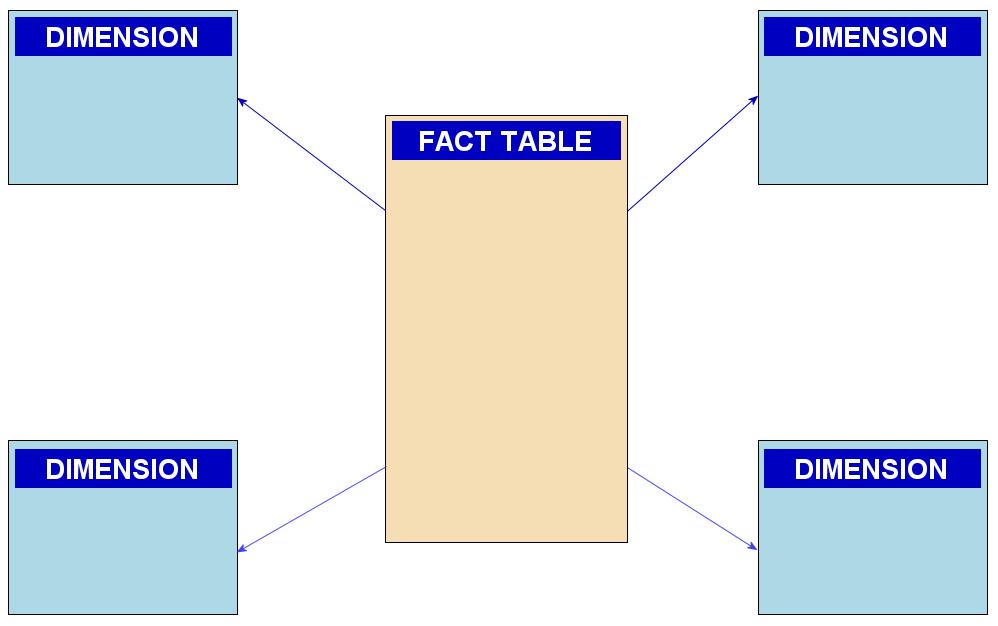
\includegraphics[width=\textwidth]{contents/img/schema_etoile.png}\\[0.1cm]
    {\small Schéma en étoile}
  \end{minipage}\hfill
  \begin{minipage}[b]{0.52\textwidth}
    \centering
    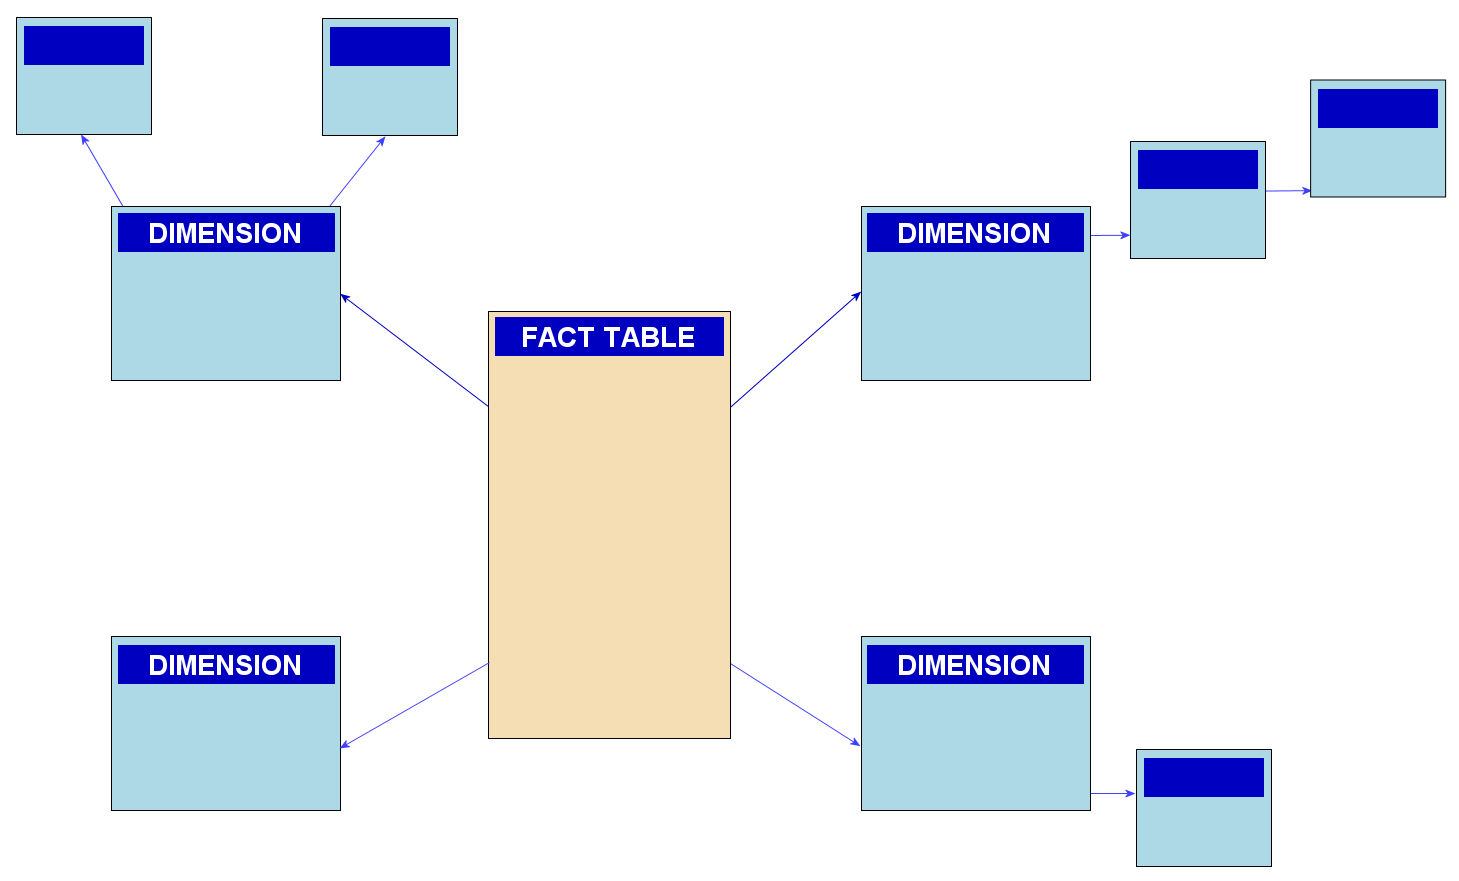
\includegraphics[width=\textwidth]{contents/img/schema_flocon.png}\\[0.1cm]
    {\small Schéma en flocon}
  \end{minipage}
\source{Wikimedia Commons, SqlPac (CC BY-SA 3.0)}
\end{center}

\begin{itemize}
	\item \textbf{Étoile}~: une table de faits entourée de dimensions dénormalisées, reliées directement à elle.
	\item \textbf{Flocon}~: les dimensions sont normalisées en sous-tables hiérarchiques (ville $\rightarrow$ département $\rightarrow$ région).
	\item \textbf{Constellation}~: plusieurs tables de faits partagent des dimensions conformes. C'est la forme d'un entrepôt construit selon Kimball.
\end{itemize}

\begin{center}
\begin{tikzpicture}[font=\scriptsize,
  fa/.style={draw=title1,thick,fill=orange!25,align=center,text width=2.6cm,minimum height=1cm,font=\scriptsize\bfseries},
  di/.style={draw=title1,thick,fill=title2!15,align=center,text width=1.9cm,minimum height=0.7cm}]
  \node[fa] (f1) at (-2.6,0) {FAIT\\CONSULTATION};
  \node[fa] (f2) at (2.6,0) {FAIT\\HOSPITALISATION};
  \node[di] (t) at (0,1.6) {Temps};
  \node[di] (p) at (0,0) {Patient};
  \node[di] (d) at (0,-1.6) {Diagnostic};
  \node[di] (pr) at (-6,0.8) {Professionnel};
  \node[di] (mu) at (-6,-0.8) {Mutuelle};
  \node[di] (e) at (6,0) {Établissement};
  \foreach \x in {t,p,d} {\draw[thick,title1] (f1) -- (\x); \draw[thick,title1] (f2) -- (\x);}
  \draw[thick,title1] (f1) -- (pr); \draw[thick,title1] (f1) -- (mu); \draw[thick,title1] (f2) -- (e);
  \node[font=\scriptsize\itshape,gray] at (0,-2.35) {dimensions conformes partagées};
\end{tikzpicture}\\[0.1cm]
{\small Schéma en constellation (exemple CHU)}
\end{center}

\begin{center}
\begin{tabularx}{\textwidth}{>{\bfseries}l >{\raggedright\arraybackslash}X >{\raggedright\arraybackslash}X >{\raggedright\arraybackslash}X}
\toprule
Critère & Étoile & Flocon & Constellation \\
\midrule
Dimensions & Dénormalisées & Normalisées & Partagées entre faits \\
Jointures & Une par dimension & Plusieurs par dimension & Une par dimension et par fait \\
Performance & Très bonne & Plus faible & Bonne \\
Redondance & Forte & Faible & Forte, mais dimensions communes \\
Lisibilité & Très simple & Plus complexe & Moyenne \\
Usage & Un data mart & Hiérarchies profondes, dimensions volumineuses & Entrepôt multi-sujets \\
\bottomrule
\end{tabularx}
\end{center}

\subsection{Choix pour le CHU}

\noindent Pour une maquette à livrer en trois semaines, l'approche de \textbf{Kimball} est la plus adaptée~: elle produit vite des data marts exploitables dans Power BI. Les sujets d'analyse (consultations, hospitalisations, satisfaction, décès) partagent le temps, les patients, les établissements et les diagnostics. On retient donc un schéma en \textbf{constellation}, en gardant chaque data mart en étoile pour limiter les jointures dans Hive.

\noindent À partir des données fournies, les tables de faits candidates sont~:

\begin{center}
\begin{tabularx}{\textwidth}{>{\bfseries}l >{\raggedright\arraybackslash}X >{\raggedright\arraybackslash}X >{\raggedright\arraybackslash}X}
\toprule
Fait & Grain & Mesures & Dimensions \\
\midrule
Consultation & Une consultation & Nombre, durée (fin $-$ début) & Temps, Patient, Professionnel, Diagnostic, Mutuelle \\
Prescription & Un médicament prescrit lors d'une consultation & Nombre de prescriptions & Temps, Patient, Médicament, Professionnel \\
Hospitalisation & Un séjour & Nombre, durée en jours & Temps (entrée), Patient, Établissement, Diagnostic \\
Satisfaction & Un établissement pour une année de recueil & Scores par thème, nombre de réponses, taux de recommandation & Temps (année), Établissement \\
Décès & Un décès & Nombre, âge au décès & Temps, Lieu (commune) \\
\bottomrule
\end{tabularx}
\end{center}

\noindent Les dimensions Temps, Patient (pseudonymisé), Établissement (code FINESS) et Diagnostic (code CIM-10) sont conformes~: une seule table de chaque, utilisée par tous les faits. Au niveau physique, les tables seront stockées dans Hive au format ORC et partitionnées par année. Chaque année devient un dossier dans HDFS. Une requête filtrée sur \texttt{annee = 2023} ne lit alors que le dossier correspondant (\textit{partition pruning}), et le format ORC, stocké par colonnes et compressé, ne lit que les colonnes utiles~:

\begin{center}
\begin{minipage}{0.62\textwidth}
\begin{tcolorbox}[colback=title2!6,colframe=title1,title=\textbf{Stockage physique dans HDFS},fonttitle=\small,boxsep=2pt]
\ttfamily\scriptsize
/user/hive/warehouse/chu.db/\\
\hspace*{1em}fait\_hospitalisation/\\
\hspace*{2em}annee=2021/\hspace*{1em}part-00000.orc\\
\hspace*{2em}annee=2022/\hspace*{1em}part-00000.orc\\
\hspace*{2em}annee=2023/\hspace*{1em}part-00000.orc\\
\hspace*{1em}dim\_etablissement/\hspace*{1em}part-00000.orc\\
\hspace*{1em}dim\_temps/\hspace*{1em}part-00000.orc
\end{tcolorbox}
\end{minipage}
\end{center}


% --- ARCHITECTURE DU PROJET CHU ---
\newpage
\section{Architecture du projet CHU}

\subsection{Schéma d'architecture d'Archie}

\noindent Le schéma fourni par Archie décrit la chaîne de traitement des données du projet CHU, des sources jusqu'à la restitution. Il est redessiné ci-dessous en couches. Les pastilles rouges renvoient aux limites relevées dans la partie suivante.

\begin{center}
\begin{tikzpicture}[font=\scriptsize,
  lay/.style={fill=title1,text=white,font=\scriptsize\bfseries,rounded corners,align=center,text width=2.1cm,minimum height=1.2cm},
  cont/.style={draw=title1!40,fill=title2!6,rounded corners},
  comp/.style={draw=title1,thick,rounded corners,fill=white,align=center,minimum height=0.8cm},
  arr/.style={-{Latex},thick,title1},
  darr/.style={{Latex}-{Latex},thick,title1},
  pin/.style={circle,fill=red!70!black,text=white,font=\tiny\bfseries,inner sep=0pt,minimum size=0.42cm}]
  \foreach \y/\lab in {0/Sources, -1.9/Data Lake, -3.8/Intégration, -5.7/{Cloudera\\(Hadoop)}, -7.6/Restitution} {
    \node[lay] at (1.2,\y) {\lab};
    \draw[cont] (2.6,{\y+0.6}) rectangle (13.4,{\y-0.6});
  }
  \node[comp,text width=2.3cm] (csv) at (4.1,0) {Fichiers CSV};
  \node[comp,text width=2.3cm] (xls) at (6.7,0) {Fichiers Excel};
  \node[comp,text width=2.3cm] (mys) at (9.3,0) {Base MySQL};
  \node[comp,text width=2.3cm] (pg) at (11.9,0) {Base PostgreSQL};
  \node[comp,text width=3cm] (hdfs) at (8,-1.9) {HDFS (Hadoop)};
  \node[comp,text width=3cm] (etl) at (8,-3.8) {ETL};
  \node[comp,text width=2.6cm] (mr) at (4.6,-5.7) {MapReduce};
  \node[comp,text width=2.6cm] (hive) at (8,-5.7) {Hive};
  \node[comp,text width=2.6cm] (bdd) at (11.4,-5.7) {Base de données};
  \node[comp,text width=3cm] (pbi) at (5.6,-7.6) {Power BI};
  \node[comp,text width=3cm] (req) at (10.4,-7.6) {Requêtes (cube OLAP)};
  \draw[darr] (8,-0.6) -- (8,-1.3);
  \draw[darr] (8,-2.5) -- (8,-3.2);
  \draw[arr] (8,-4.4) -- (8,-5.1);
  \draw[arr] (8,-6.3) -- (8,-7.0);
  \node[pin] at (8.45,-0.95) {1};
  \node[pin] at (mys.north east) {2};
  \node[pin] at (xls.north east) {2};
  \node[pin] at (hdfs.north east) {3};
  \node[pin] at (etl.north east) {4};
  \node[pin] at (bdd.north east) {5};
  \node[pin] at (8.45,-6.65) {6};
\end{tikzpicture}\\[0.1cm]
{\small Schéma d'Archie, redessiné}
\end{center}

\noindent L'architecture se lit de haut en bas, en cinq couches~:
\begin{enumerate}
	\item \textbf{Sources de données}~: des fichiers plats (CSV, Excel) et des bases relationnelles (MySQL, PostgreSQL), qui représentent les systèmes existants du CHU.
	\item \textbf{Data Lake (HDFS Hadoop)}~: les données sont collectées brutes dans le système de fichiers distribué de Hadoop, qui les découpe en blocs répliqués sur les nœuds du cluster.
	\item \textbf{ETL}~: les données sont extraites du Data Lake, nettoyées, transformées puis chargées dans l'entrepôt.
	\item \textbf{Stockage et traitement (Cloudera / Hadoop)}~: l'entrepôt de données est hébergé sur la plateforme Cloudera. Hive expose les données en SQL, et MapReduce exécute les traitements distribués.
	\item \textbf{Restitution}~: Power BI produit les tableaux de bord, et les requêtes multidimensionnelles (cube OLAP) répondent aux analyses du cahier des charges.
\end{enumerate}

\subsection{Limites du schéma}

\noindent Le principe général (sources, Data Lake, ETL, entrepôt, restitution) est correct, mais le schéma présente plusieurs erreurs ou manques~:
\begin{enumerate}
	\item \textbf{Flèches bidirectionnelles.} Les sources, HDFS et l'ETL sont reliés par des doubles flèches. Une chaîne décisionnelle lit les sources sans jamais les modifier~: le flux doit aller dans un seul sens.
	\item \textbf{Sources inexactes.} Les données fournies («~DATA 2024~») ne contiennent aucune base MySQL, et un seul fichier Excel, simple doublon d'un CSV de satisfaction. On dispose d'une sauvegarde PostgreSQL (patients, consultations, prescriptions, médicaments, mutuelles) et de fichiers CSV (hospitalisations, établissements et professionnels de santé, décès, satisfaction).
	\item \textbf{HDFS isolé de Cloudera.} HDFS fait partie de la distribution Cloudera. Le Data Lake et l'entrepôt sont hébergés sur le même cluster, ce que le schéma ne montre pas.
	\item \textbf{ETL non défini.} L'outil n'est pas nommé et son rôle se limite à un passage. Dans le projet, c'est \textbf{Talend Open Studio for Big Data}, et c'est à cette étape que les données doivent être pseudonymisées.
	\item \textbf{Entrepôt non identifié.} «~Base de données~» ne dit pas où se trouve l'entrepôt ni comment il est modélisé. Il faut des tables Hive organisées en data marts dimensionnels.
	\item \textbf{Restitution lente.} Power BI interrogerait Hive, qui exécute des traitements MapReduce écrits sur disque~: plusieurs dizaines de secondes par requête. Pour des tableaux de bord interactifs, Impala est plus adapté.
	\item \textbf{Aucune sécurité ni conformité.} Rien n'apparaît sur le RGPD, l'hébergement HDS, l'authentification ou les droits d'accès, alors que les données sont des données de santé.
	\item \textbf{Aucune planification.} Le schéma ne montre pas comment et quand les chargements sont déclenchés.
\end{enumerate}

\subsection{Proposition d'architecture}

\noindent L'architecture proposée corrige ces points. Elle est hybride~: un Data Lake HDFS pour le stockage et un entrepôt Hive en constellation pour l'analyse. Elle repose sur les outils de l'environnement virtualisé (machine Cloudera QuickStart CDH~5.12, Talend Open Studio for Big Data, Power BI). Le schéma est présenté page suivante.

\begin{center}
\begin{tabularx}{\textwidth}{>{\bfseries}l l >{\raggedright\arraybackslash}X}
\toprule
Couche & Outil & Rôle \\
\midrule
Sources & PostgreSQL, CSV & Données de gestion du CHU et données publiques (établissements, décès, satisfaction) \\
Intégration & Talend Open Studio for Big Data & Extraire, contrôler, pseudonymiser puis déposer les données dans HDFS \\
Data Lake & HDFS & Conserver les données brutes (pseudonymisées) et préparées, répliquées sur le cluster \\
Entrepôt & Hive & Tables dimensionnelles en constellation, au format ORC partitionné \\
Accès & Hive, Impala & Hive pour les traitements lourds, Impala pour les requêtes interactives \\
Restitution & Power BI, Hue & Tableaux de bord des décideurs, requêtes des analystes \\
Transverse & Kerberos, Sentry, HDS & Sécurité, droits d'accès, conformité RGPD \\
\bottomrule
\end{tabularx}
\end{center}

\needspace{8\baselineskip}
\noindent \textbf{Ce qui change par rapport au schéma d'Archie}~:
\begin{itemize}
	\item le flux est à sens unique, des sources vers la restitution~;
	\item les sources correspondent aux données réellement fournies~;
	\item Talend est placé avant HDFS~: les données sont pseudonymisées avant d'être stockées, et aucune donnée directement identifiante n'est écrite dans HDFS~;
	\item le Data Lake est découpé en une zone brute et une zone préparée, toutes deux dans le cluster Cloudera~;
	\item l'entrepôt est explicite~: des data marts Hive en constellation~;
	\item Impala sert les tableaux de bord, Hive reste pour les traitements batch~;
	\item sécurité, conformité et planification deviennent des couches transverses.
\end{itemize}

\begin{landscape}
\thispagestyle{fancy}
\begin{center}
\hyphenpenalty=10000 \exhyphenpenalty=10000
\begin{tikzpicture}[font=\scriptsize,
  grp/.style={draw=gray!70,dashed,thick,rounded corners,fill=#1},
  grp/.default={gray!4},
  glab/.style={anchor=north west,font=\small\bfseries,text=title1},
  box/.style={draw=#1,thick,rounded corners,fill=white,align=center,text width=2.8cm,minimum height=1cm},
  box/.default={gray!70},
  tal/.style={draw=orange!80!black,thick,rounded corners,fill=orange!15,align=center,text width=3cm,minimum height=1.5cm},
  cyl/.style={cylinder,shape border rotate=90,aspect=0.15,draw=title1,thick,fill=#1,align=center,text width=2.6cm,minimum height=2.9cm},
  cyl/.default={title2!12},
  arr/.style={-{Latex},very thick,gray!70!black}]

  % cadres
  \draw[grp] (0,0) rectangle (3.6,-9.0);
  \node[glab] at (0.1,-0.1) {1. Sources};
  \draw[grp=orange!4] (4.3,0) rectangle (7.9,-9.0);
  \node[glab] at (4.4,-0.1) {2. Intégration};
  \draw[grp=title2!4] (8.6,0) rectangle (19.4,-9.0);
  \node[glab] at (8.7,-0.1) {Cluster Cloudera CDH (VM)};
  \draw[grp] (19.9,0) rectangle (24.0,-9.0);
  \node[glab] at (20.0,-0.1) {6. Restitution};

  % 1. sources
  \node[cyl=white,draw=gray!70,text width=2.7cm,minimum height=1.9cm] (pg) at (1.8,-2.15) {\textbf{PostgreSQL}\\ DATA2023~: patients, consultations, prescriptions};
  \node[box] (c1) at (1.8,-3.9) {\textbf{CSV}\\ hospitalisations};
  \node[box] (c2) at (1.8,-5.3) {\textbf{CSV}\\ établissements et professionnels};
  \node[box] (c3) at (1.8,-6.7) {\textbf{CSV}\\ décès (25~M lignes)};
  \node[box] (c4) at (1.8,-8.1) {\textbf{CSV}\\ satisfaction (e-Satis)};

  % 2. talend
  \node[tal] (t1) at (6.1,-2.2) {\textbf{Extraction}\\ connecteurs PostgreSQL et CSV};
  \node[tal] (t2) at (6.1,-4.6) {\textbf{Nettoyage}\\ contrôle qualité, tranches d'âge, clés de substitution};
  \node[tal,fill=red!12,draw=red!60!black] (t3) at (6.1,-7.0) {\textbf{Pseudonymisation RGPD}\\ hachage salé des identifiants, identité supprimée};
  \draw[arr] (t1) -- (t2);
  \draw[arr] (t2) -- (t3);
  \foreach \s in {pg,c1,c2,c3,c4} \draw[very thick,gray!70!black] (\s.east) -- (\s.east -| 3.95,0);
  \draw[very thick,gray!70!black] (3.95,-2.15) -- (3.95,-8.1);
  \draw[arr] (3.95,-2.2) -- (t1.west);

  % cluster : data lake et entrepôt
  \node[cyl] (z1) at (10.15,-3.3) {\textbf{3. Data Lake HDFS}\\ zone brute\\[0.05cm] données pseudonymisées, format d'origine, accès restreint};
  \node[cyl] (z2) at (13.45,-3.3) {\textbf{3. Data Lake HDFS}\\ zone préparée\\[0.05cm] fichiers ORC partitionnés par année};
  \node[cyl=orange!12,draw=orange!80!black,text width=3cm] (dw) at (17.0,-3.3) {\textbf{4. Entrepôt Hive}\\ constellation\\[0.05cm] data marts consultations, hospitalisations, satisfaction, décès};
  \draw[arr] (t3.east) -- (8.25,-7.0) |- (z1.west);
  \draw[arr] (z1) -- node[above,font=\tiny]{Talend / Hive} (z2);
  \draw[arr] (z2) -- (dw);

  % accès aux données
  \node[box=title1,text width=4.4cm] (hv) at (11.8,-7.3) {\textbf{5. Hive (HiveQL $\rightarrow$ MapReduce)}\\ traitements batch au plus près des données (colocalisation)};
  \node[box=title1,text width=3cm] (imp) at (17.0,-7.3) {\textbf{5. Impala}\\ requêtes SQL interactives};
  \draw[arr] (dw.south) -- (imp.north);
  \draw[arr] (dw.south) -- ++(0,-0.6) -| (hv.north);

  % 6. restitution
  \node[box=yellow!60!black,fill=yellow!20,text width=3.2cm] (pbi) at (21.95,-2.2) {\textbf{Power BI}\\ connecteur Impala (ODBC), mesures DAX calculées à la volée};
  \node[box,text width=3.2cm] (usr) at (21.95,-4.6) {\textbf{Utilisateurs CHU}\\ tableaux de bord, données agrégées non nominatives};
  \node[box,text width=3.2cm] (hue) at (21.95,-7.3) {\textbf{Hue}\\ requêtes ad hoc des analystes};
  \draw[arr] (imp.east) -- node[below,font=\tiny]{ODBC} (19.6,-7.3) |- (pbi.west);
  \draw[arr] (pbi) -- (usr);
  \draw[arr] (hv.south) |- (19.75,-8.65) |- ([yshift=-0.3cm]hue.west);

  % transverse
  \node[draw=red!60!black,thick,rounded corners,fill=red!5,text width=23.6cm,align=left,anchor=north west,inner sep=0.2cm] at (0,-9.4) {%
    \textbf{Sécurité et RGPD (transverse)}~: hébergement certifié HDS~· authentification Kerberos~· droits par rôle (Sentry)~· chiffrement des données~· journalisation des accès~· durées de conservation par zone.\\
    Les identifiants directs (nom, prénom, n° de sécurité sociale, adresse, date de naissance) sont pseudonymisés par Talend avant d'être écrits dans HDFS~: seules des données pseudonymisées puis agrégées atteignent l'entrepôt et Power BI.\\
    \textbf{Orchestration}~: jobs Talend planifiés (chargement nocturne).};
\end{tikzpicture}\\[0.2cm]
{\small Architecture proposée~: Data Lake et entrepôt sur le cluster Cloudera}
\end{center}
\end{landscape}

\subsection{Contraintes RGPD sur les données}

\noindent Les données du projet sont des données de santé, classées comme données sensibles par le RGPD (article 9). Le tableau suivant recense les données personnelles de chaque source et le traitement prévu dans Talend~:

\begin{center}
\small
\begin{tabularx}{\textwidth}{>{\bfseries\raggedright\arraybackslash}p{3cm} >{\raggedright\arraybackslash}X >{\raggedright\arraybackslash}X}
\toprule
Source & Données personnelles & Traitement \\
\midrule
Patient (PostgreSQL) & Nom, prénom, adresse, e-mail, téléphone, numéro de sécurité sociale, date de naissance & Identifiant remplacé par un hachage salé, colonnes d'identité supprimées, date de naissance réduite à une tranche d'âge, adresse réduite au département \\
Consultation, prescription, hospitali\-sation & Diagnostics, médicaments, durées de séjour (données de santé) & Conservés, mais rattachés au seul identifiant pseudonymisé \\
Professionnels de santé & Nom, prénom, profession, commune & Données publiques (annuaire RPPS)~; seuls l'identifiant, la profession et la spécialité sont nécessaires \\
Décès & Nom, prénom, date et lieu de naissance et de décès & Fichier public de l'INSEE~; utilisé pour des statistiques agrégées, sans les noms \\
Satisfaction & Aucune (résultats agrégés par établissement) & Aucun traitement particulier \\
\bottomrule
\end{tabularx}
\end{center}

\noindent Les autres principes du RGPD se traduisent ainsi dans l'architecture~:
\begin{itemize}
	\item \textbf{finalité}~: les données ne servent qu'au pilotage de l'activité hospitalière décrit dans le cahier des charges~;
	\item \textbf{minimisation}~: seules les colonnes utiles aux analyses sont chargées (le groupe sanguin, le poids ou la taille ne le sont que si un indicateur les utilise)~;
	\item \textbf{conservation}~: une durée est fixée pour chaque zone, et les partitions par année permettent de supprimer facilement les données expirées~;
	\item \textbf{sécurité}~: hébergement HDS, authentification Kerberos, droits par rôle et journalisation des accès~;
	\item \textbf{droits des personnes}~: la table de correspondance entre identifiant réel et pseudonyme reste dans le système source, hors du cluster, ce qui permet de traiter une demande d'accès ou d'effacement.
\end{itemize}

\noindent La pseudonymisation n'est pas une anonymisation~: les données restent personnelles au sens du RGPD. Seuls les indicateurs agrégés publiés dans Power BI, avec des effectifs suffisants, peuvent être considérés comme anonymes.

% --- CONCLUSION ---
\newpage
\section*{Conclusion}
\phantomsection
\addcontentsline{toc}{section}{Conclusion}

\noindent \textbf{En réponse à la problématique}, valider une architecture Big Data performante pour le projet CHU a d'abord demandé de corriger le schéma d'Archie. Son principe général (sources, Data Lake, ETL, entrepôt, restitution) est juste, mais les flux sont à double sens, les sources ne correspondent pas aux données fournies, l'entrepôt n'est pas identifié et rien ne traite la sécurité ni le RGPD.

\vspace{0.2cm}

\noindent L'architecture proposée est \textbf{hybride}. \textbf{Talend} extrait les données PostgreSQL et CSV, les contrôle et les \textbf{pseudonymise avant tout stockage}. \textbf{HDFS} conserve ces données dans une zone brute puis une zone préparée, répliquées sur le cluster Cloudera. \textbf{Hive} les organise en data marts. \textbf{Impala} sert les requêtes interactives de \textbf{Power BI}, et Hive reste pour les traitements batch exécutés en MapReduce au plus près des données. La sécurité (hébergement HDS, Kerberos, droits par rôle, journalisation) et la planification des chargements sont des couches transverses.

\vspace{0.2cm}

\noindent Pour le modèle logique, l'étude des approches de modélisation conduit à retenir celle de \textbf{Kimball}, sous la forme d'une \textbf{constellation}~: des tables de faits (consultations, hospitalisations, satisfaction, décès) qui partagent des dimensions conformes (temps, patient pseudonymisé, établissement, diagnostic). Ce modèle est rapide à mettre en place, lisible pour les utilisateurs et performant en lecture, ce qui convient à une maquette à livrer en trois semaines.

\vspace{0.2cm}

\noindent La suite du projet consiste à finaliser le modèle dimensionnel détaillé, puis à passer à l'intégration des données avec Talend, à l'implémentation physique dans Hive et à la construction des tableaux de bord dans Power BI.

% --- CAPITALISATION ---
\newpage
\section*{Capitalisation}
\phantomsection
\addcontentsline{toc}{section}{Capitalisation}

\begin{center}
\small
\setlength{\tabcolsep}{8pt}
\renewcommand{\arraystretch}{1.15}

\begin{tabular}{|>{\raggedright\arraybackslash}p{0.30\textwidth}|>{\raggedright\arraybackslash}p{0.47\textwidth}|m{0.08\textwidth}|}
\hline
\textbf{AAV} & \textbf{Commentaire} & \textbf{Statut} \\ \hline

Identifier les contraintes sur les données liées au RGPD &
Données personnelles recensées source par source (identité des patients, données de santé, fichier des décès) avec le traitement prévu~: pseudonymisation, minimisation, conservation, hébergement HDS. &
{\color{green!60!black}Acquis} \\ \hline

Interpréter les 5V du Big Data &
Volume, vélocité, variété, véracité et valeur définis et illustrés par les données de santé du CHU. &
{\color{green!60!black}Acquis} \\ \hline

Décrire une architecture Big Data &
Schéma d'Archie analysé, huit limites relevées, puis architecture corrigée proposée (Talend, HDFS, Hive, Impala, Power BI) et justifiée couche par couche. &
{\color{green!60!black}Acquis} \\ \hline

Décrire une infrastructure de stockage distribuée (cluster de serveurs, virtualisation, NAS vs SAN, \dots) &
Cluster et scalabilité horizontale, virtualisation et localité des données, comparaison DAS / NAS / SAN. &
{\color{green!60!black}Acquis} \\ \hline

Décrire l'utilisation du cloud dans le cadre du stockage de données &
Modèles IaaS, PaaS, SaaS et de déploiement, stockage objet, avantages et limites, contrainte HDS pour les données de santé. &
{\color{green!60!black}Acquis} \\ \hline

Présenter le traitement de données de manière distribuée (exemple~: MapReduce) &
Étapes Map, Shuffle \& Sort et Reduce illustrées par le comptage des consultations par diagnostic, et lien avec les requêtes Hive. &
{\color{green!60!black}Acquis} \\ \hline

Décrire le fonctionnement des systèmes de fichiers distribués &
Architecture de HDFS (NameNode, DataNodes), découpage en blocs, réplication et tolérance aux pannes. &
{\color{green!60!black}Acquis} \\ \hline

Décrire le fonctionnement d'une application d'entreposage de données &
OLTP et OLAP comparés, chaîne ETL, zone de préparation, entrepôt, data marts et restitution. &
{\color{green!60!black}Acquis} \\ \hline

Concevoir un modèle dimensionnel (Data Mart) &
Approches Inmon, Kimball et Data Vault comparées, schémas étoile, flocon et constellation étudiés, faits et dimensions du CHU identifiés. Le modèle détaillé reste à finaliser. &
{\color{orange}Partiel} \\ \hline

Identifier les difficultés associées aux traitements distribués &
Pannes, réseau, déséquilibre de charge, théorème CAP, latence de MapReduce, petits fichiers, complexité et sécurité. &
{\color{green!60!black}Acquis} \\ \hline

\end{tabular}
\end{center}

% --- RESSOURCES ---
\newpage
\section*{Ressources}
\phantomsection
\addcontentsline{toc}{section}{Ressources}

\begin{itemize}
	\item \textbf{Documentation Apache Hadoop (HDFS, MapReduce)} : \url{https://hadoop.apache.org/docs/stable/}
	\item \textbf{Apache Hive} : \url{https://hive.apache.org/}
	\item \textbf{Apache Impala} : \url{https://impala.apache.org/}
	\item \textbf{Documentation Cloudera} : \url{https://docs.cloudera.com/}
	\item \textbf{Documentation Talend} : \url{https://help.talend.com/}
	\item \textbf{Documentation Power BI} : \url{https://learn.microsoft.com/fr-fr/power-bi/}
	\item \textbf{Techniques de modélisation dimensionnelle (Kimball Group)} : \url{https://www.kimballgroup.com/data-warehouse-business-intelligence-resources/kimball-techniques/dimensional-modeling-techniques/}
	\item \textbf{RGPD (CNIL)} : \url{https://www.cnil.fr/fr/reglement-europeen-protection-donnees}
	\item \textbf{Hébergement de données de santé (HDS)} : \url{https://esante.gouv.fr/produits-services/hds}
	\item \textbf{Fichier des personnes décédées (INSEE, data.gouv.fr)} : \url{https://www.data.gouv.fr/fr/datasets/fichier-des-personnes-decedees/}
\end{itemize}
